\documentclass{ximera}

%\usepackage{todonotes}

\newcommand{\todo}{}

\usepackage{tkz-euclide}
\tikzset{>=stealth} %% cool arrow head
\tikzset{shorten <>/.style={ shorten >=#1, shorten <=#1 } } %% allows shorter vectors

\usepackage{tkz-tab}  %% sign charts
\usetikzlibrary{decorations.pathreplacing} 

\usetikzlibrary{backgrounds} %% for boxes around graphs
\usetikzlibrary{shapes,positioning}  %% Clouds and stars
\usetikzlibrary{matrix} %% for matrix
\usepgfplotslibrary{polar} %% for polar plots
\usetkzobj{all}
\usepackage[makeroom]{cancel} %% for strike outs
%\usepackage{mathtools} %% for pretty underbrace % Breaks Ximera
\usepackage{multicol}

\usepackage{polynom}



\usepackage[many]{tcolorbox}  %% for titled boxes
\newtcolorbox{xbox}[1]{%
    tikznode boxed title,
    enhanced,
    arc=0mm,
    interior style={white},
    attach boxed title to top center= {yshift=-\tcboxedtitleheight/2},
    fonttitle=\bfseries,
    colbacktitle=white,coltitle=black,
    boxed title style={size=normal,colframe=white,boxrule=0pt},
    title={#1}}


\usepackage{array}
\setlength{\extrarowheight}{+.1cm}   
\newdimen\digitwidth
\settowidth\digitwidth{9}
\def\divrule#1#2{
\noalign{\moveright#1\digitwidth
\vbox{\hrule width#2\digitwidth}}}





\newcommand{\RR}{\mathbb R}
\newcommand{\R}{\mathbb R}
\newcommand{\N}{\mathbb N}
\newcommand{\Z}{\mathbb Z}

%\renewcommand{\d}{\,d\!}
\renewcommand{\d}{\mathop{}\!d}
\newcommand{\dd}[2][]{\frac{\d #1}{\d #2}}
\newcommand{\pp}[2][]{\frac{\partial #1}{\partial #2}}
\renewcommand{\l}{\ell}
\newcommand{\ddx}{\frac{d}{\d x}}
\newcommand{\ddt}{\frac{d}{\d t}}

\newcommand{\zeroOverZero}{\ensuremath{\boldsymbol{\tfrac{0}{0}}}}
\newcommand{\inftyOverInfty}{\ensuremath{\boldsymbol{\tfrac{\infty}{\infty}}}}
\newcommand{\zeroOverInfty}{\ensuremath{\boldsymbol{\tfrac{0}{\infty}}}}
\newcommand{\zeroTimesInfty}{\ensuremath{\small\boldsymbol{0\cdot \infty}}}
\newcommand{\inftyMinusInfty}{\ensuremath{\small\boldsymbol{\infty - \infty}}}
\newcommand{\oneToInfty}{\ensuremath{\boldsymbol{1^\infty}}}
\newcommand{\zeroToZero}{\ensuremath{\boldsymbol{0^0}}}
\newcommand{\inftyToZero}{\ensuremath{\boldsymbol{\infty^0}}}



\newcommand{\numOverZero}{\ensuremath{\boldsymbol{\tfrac{\#}{0}}}}
\newcommand{\dfn}{\textbf}
%\newcommand{\unit}{\,\mathrm}
\newcommand{\unit}{\mathop{}\!\mathrm}
\newcommand{\eval}[1]{\bigg[ #1 \bigg]}
\newcommand{\seq}[1]{\left( #1 \right)}
\renewcommand{\epsilon}{\varepsilon}
\renewcommand{\iff}{\Leftrightarrow}

\DeclareMathOperator{\arccot}{arccot}
\DeclareMathOperator{\arcsec}{arcsec}
\DeclareMathOperator{\arccsc}{arccsc}
\DeclareMathOperator{\si}{Si}
\DeclareMathOperator{\proj}{proj}
\DeclareMathOperator{\scal}{scal}


\newcommand{\tightoverset}[2]{% for arrow vec
  \mathop{#2}\limits^{\vbox to -.5ex{\kern-0.75ex\hbox{$#1$}\vss}}}
\newcommand{\arrowvec}[1]{\tightoverset{\scriptstyle\rightharpoonup}{#1}}
\renewcommand{\vec}{\mathbf}
\newcommand{\veci}{\vec{i}}
\newcommand{\vecj}{\vec{j}}
\newcommand{\veck}{\vec{k}}
\newcommand{\vecl}{\boldsymbol{\l}}

\newcommand{\dotp}{\bullet}
\newcommand{\cross}{\boldsymbol\times}
\newcommand{\grad}{\boldsymbol\nabla}
\newcommand{\divergence}{\grad\dotp}
\newcommand{\curl}{\grad\cross}
%\DeclareMathOperator{\divergence}{divergence}
%\DeclareMathOperator{\curl}[1]{\grad\cross #1}


\colorlet{textColor}{black} 
\colorlet{background}{white}
\colorlet{penColor}{blue!50!black} % Color of a curve in a plot
\colorlet{penColor2}{red!50!black}% Color of a curve in a plot
\colorlet{penColor3}{red!50!blue} % Color of a curve in a plot
\colorlet{penColor4}{green!50!black} % Color of a curve in a plot
\colorlet{penColor5}{orange!80!black} % Color of a curve in a plot
\colorlet{fill1}{penColor!20} % Color of fill in a plot
\colorlet{fill2}{penColor2!20} % Color of fill in a plot
\colorlet{fillp}{fill1} % Color of positive area
\colorlet{filln}{penColor2!20} % Color of negative area
\colorlet{fill3}{penColor3!20} % Fill
\colorlet{fill4}{penColor4!20} % Fill
\colorlet{fill5}{penColor5!20} % Fill
\colorlet{gridColor}{gray!50} % Color of grid in a plot

\newcommand{\surfaceColor}{violet}
\newcommand{\surfaceColorTwo}{redyellow}
\newcommand{\sliceColor}{greenyellow}




\pgfmathdeclarefunction{gauss}{2}{% gives gaussian
  \pgfmathparse{1/(#2*sqrt(2*pi))*exp(-((x-#1)^2)/(2*#2^2))}%
}


%%%%%%%%%%%%%
%% Vectors
%%%%%%%%%%%%%

%% Simple horiz vectors
\renewcommand{\vector}[1]{\left\langle #1\right\rangle}


%% %% Complex Horiz Vectors with angle brackets
%% \makeatletter
%% \renewcommand{\vector}[2][ , ]{\left\langle%
%%   \def\nextitem{\def\nextitem{#1}}%
%%   \@for \el:=#2\do{\nextitem\el}\right\rangle%
%% }
%% \makeatother

%% %% Vertical Vectors
%% \def\vector#1{\begin{bmatrix}\vecListA#1,,\end{bmatrix}}
%% \def\vecListA#1,{\if,#1,\else #1\cr \expandafter \vecListA \fi}

%%%%%%%%%%%%%
%% End of vectors
%%%%%%%%%%%%%

%\newcommand{\fullwidth}{}
%\newcommand{\normalwidth}{}



%% makes a snazzy t-chart for evaluating functions
%\newenvironment{tchart}{\rowcolors{2}{}{background!90!textColor}\array}{\endarray}

%%This is to help with formatting on future title pages.
\newenvironment{sectionOutcomes}{}{} 



%% Flowchart stuff
%\tikzstyle{startstop} = [rectangle, rounded corners, minimum width=3cm, minimum height=1cm,text centered, draw=black]
%\tikzstyle{question} = [rectangle, minimum width=3cm, minimum height=1cm, text centered, draw=black]
%\tikzstyle{decision} = [trapezium, trapezium left angle=70, trapezium right angle=110, minimum width=3cm, minimum height=1cm, text centered, draw=black]
%\tikzstyle{question} = [rectangle, rounded corners, minimum width=3cm, minimum height=1cm,text centered, draw=black]
%\tikzstyle{process} = [rectangle, minimum width=3cm, minimum height=1cm, text centered, draw=black]
%\tikzstyle{decision} = [trapezium, trapezium left angle=70, trapezium right angle=110, minimum width=3cm, minimum height=1cm, text centered, draw=black]


\outcome{Use ``shortcut'' rules to find and use derivatives.}
\outcome{Use the definition of the derivative to develop a shortcut
  rule to find the derivative of the natural exponential function.}

\title[Dig-In:]{The derivative of the natural exponential function}

\begin{document}
\begin{abstract}
  We derive the derivative of the natural exponential function.
\end{abstract}
\maketitle

We don't know anything about derivatives that allows us to compute the
derivatives of exponential functions without getting our hands
dirty. Let's do a little work with the definition of the derivative:
\begin{explanation}
\begin{align*}
\ddx a^x &=\lim_{h\to 0} \frac{a^{x+h}-a^x}{h} \\
&=\lim_{h\to 0} \frac{a^xa^{h}-a^x}{h} \\
&=\lim_{h\to 0} a^x\frac{\answer[given]{a^{h}-1}}{h} \\
&=a^x\lim_{h\to 0} \frac{a^{h}-1}{h} \\
&=a^x \cdot \underbrace{\text{(constant)}}_{\lim_{h\to 0} \frac{a^{h}-1}{h}}
\end{align*}
\end{explanation}
There are two interesting things to note here: We are left with a
limit that involves $h$ but not $x$, which means that whatever $
\lim_{h\to 0} (a^h-1)/h$ is, we know that it is a number, or in other words, a
constant. This means that $a^x$ has a remarkable property:
\begin{quote}
  \textbf{The derivative of an exponential function is a constant
    times itself.}
\end{quote}
Unfortunately it is beyond the scope of this text to compute the limit
\[
\lim_{h\to 0} \frac{a^h-1}{h}.
\]
However, we can look at some examples. Consider $(2^h-1)/h$ and $(3^h-1)/h$:

\begin{image}
  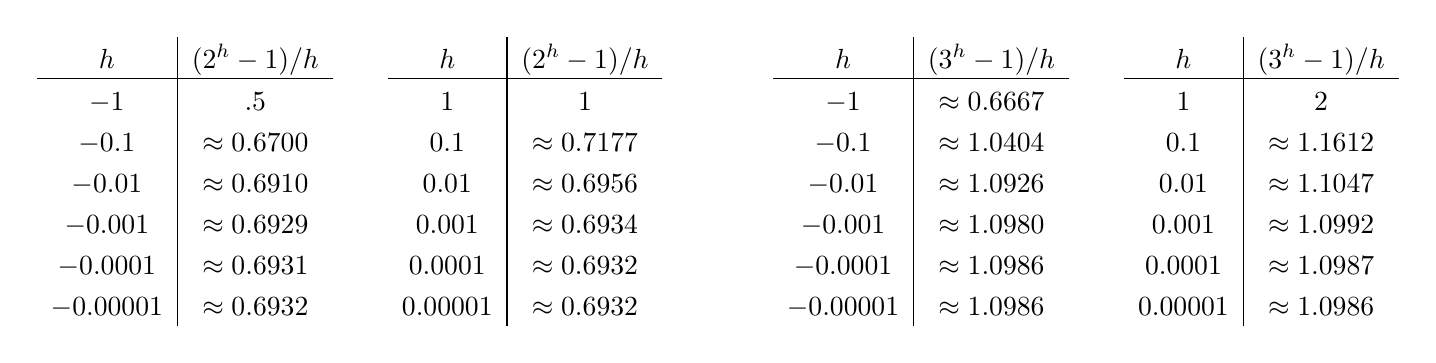
\begin{tikzpicture}
    \node at (0,0) {$\begin{array}{c|c}
 h &     (2^h-1)/h\\ \hline
 -1 & .5  \\
-0.1 &  \approx0.6700 \\
-0.01 & \approx0.6910 \\
-0.001 & \approx0.6929 \\
-0.0001 & \approx0.6931 \\
-0.00001 & \approx0.6932 \\
\end{array}
\qquad
\begin{array}{c|c}
 h &     (2^h-1)/h\\ \hline
 1 & 1  \\
 0.1 &  \approx0.7177 \\
 0.01 & \approx0.6956 \\
 0.001 & \approx0.6934 \\
 0.0001 & \approx0.6932 \\
 0.00001 & \approx0.6932 \\
\end{array}
\qquad\qquad
\begin{array}{c|c}
 h &     (3^h-1)/h\\ \hline
-1 & \approx 0.6667  \\
-0.1 &  \approx1.0404  \\
-0.01 & \approx1.0926 \\
-0.001 & \approx1.0980 \\
-0.0001 & \approx1.0986 \\
-0.00001 & \approx1.0986 \\
\end{array}
\qquad
\begin{array}{c|c}
 h &     (3^h-1)/h\\ \hline
 1 & 2  \\
 0.1 &  \approx1.1612 \\
 0.01 & \approx1.1047 \\
 0.001 & \approx1.0992 \\
 0.0001 & \approx1.0987 \\
 0.00001 & \approx1.0986 \\
 \end{array}$};
\end{tikzpicture}
\end{image}



While these tables don't prove that we have a pattern, it turns out that
\[
\lim_{h\to 0}\frac{2^h-1}{h} \approx .7 \qquad\text{and}\qquad \lim_{h\to 0} \frac{3^h-1}{h} \approx 1.1.
\]
Moreover, if you do more examples, choosing other values for the 
base $a$, you will find that the limit varies
directly with the value of $a$: bigger $a$, bigger limit; smaller $a$,
smaller limit. As we can already see, some of these limits will be
less than $1$ and some larger than $1$. Somewhere between $a=2$ and $a=3$
the limit will be exactly $1$. This happens when 
\[
a = e = 2.718281828459045\dots.
\]
We will define the number $e$ by this property, see the next
definition:
\begin{definition}\index{e@$e$}
  The number denoted by $e$, called \dfn{Euler's number}, is defined
  to be the number satisfying the following relation
  \[
  \lim_{h\to 0} \frac{e^h-1}{h} = 1.
  \]
\end{definition}
Using this definition, we see that the function $e^x$ has the following truly remarkable property.

\begin{theorem}[The derivative of the natural exponential function]\index{ex@$e^x$}\index{derivative!of ex@of $e^x$}
The derivative of the natural exponential function is the natural exponential function itself.  In other words,
\[
\ddx e^x = e^x.
\]
\begin{explanation}  
From the limit definition of the derivative, write
\begin{align*}
\ddx e^x&=\lim_{h\to 0} \frac{e^{x+h}-e^x}{h} \\
&=\lim_{h\to 0} \frac{e^xe^{h}-e^x}{h} \\
&=\lim_{h\to 0} \answer[given]{e^x}\frac{e^{h}-1}{h} \\
&=e^x\lim_{h\to 0} \frac{e^{h}-1}{h} \\
&=e^x.
\end{align*}
\end{explanation}
\end{theorem}


Hence $e^x$ is its own derivative. In other words, the slope of the
plot of $e^x$ is the same as its height, or the same as its second
coordinate.  Said another way, the function $f(x)=e^x$ goes through the point $(a,e^a)$
and has slope $e^a$ at that point, no matter what $a$ is. 

\begin{question}
  What is the slope of the tangent line to the function $f(x) = e^x$ at $x = 5$?
  \begin{prompt}
    The slope is $\answer[given]{e^5}$.
  \end{prompt}
\end{question}



\begin{example}
Compute:
\[
\ddx\left(8\sqrt{x} + 7e^x \right)
\]
	\begin{explanation}
		Write with me:
		\begin{align*}
			\ddx\left(8\sqrt{x} + 7e^x \right) &= 8\ddx x^{1/2} + 7\ddx e^x\\
				&= 4x^{-1/2} + 7 \answer[given]{e^x}.
		\end{align*}
	\end{explanation}
\end{example}




\begin{example}
	Compute: \[ \ddx e^{4x\sqrt{x+1}} \]
	\begin{explanation}
		We know the derivative of $e^x$, but we're being asked the derivative of $e^{4x \sqrt{x+1}}$.  The $x$ has been replaced by a function of $x$.
		We think of $e^{4x \sqrt{x+1}}$ as a composite function with $f(x) = e^x$ and $g(x) = 4x \sqrt{x+1}$.
		To take the derivative of a composite function, we have chain rule: $\ddx f(g(x)) = f'( g(x) ) g'(x)$.  
		
		We know $f'(x) = \ddx e^x = e^x$ and $g'(x) = \ddx \left( 4x \sqrt{x+1} \right)$ which we calculate by product rule as
		$4 \sqrt{x+1} + 4x \dfrac{1}{2 \sqrt{x+1}} \cdot 1$ (where we used chain rule AGAIN inside the square root).
		Our answer is then:
		\[ e^{4x \sqrt{x+1}}\left( 4\sqrt{x+1} + \dfrac{2x}{\sqrt{x+1}}\right).\]
	\end{explanation}	
\end{example}





\end{document}
